\documentclass[twoside]{book}

% Packages required by doxygen
\usepackage{fixltx2e}
\usepackage{calc}
\usepackage{doxygen}
\usepackage[export]{adjustbox} % also loads graphicx
\usepackage{graphicx}
\usepackage[utf8]{inputenc}
\usepackage{makeidx}
\usepackage{multicol}
\usepackage{multirow}
\PassOptionsToPackage{warn}{textcomp}
\usepackage{textcomp}
\usepackage[nointegrals]{wasysym}
\usepackage[table]{xcolor}

% Font selection
\usepackage[T1]{fontenc}
\usepackage[scaled=.90]{helvet}
\usepackage{courier}
\usepackage{amssymb}
\usepackage{sectsty}
\renewcommand{\familydefault}{\sfdefault}
\allsectionsfont{%
  \fontseries{bc}\selectfont%
  \color{darkgray}%
}
\renewcommand{\DoxyLabelFont}{%
  \fontseries{bc}\selectfont%
  \color{darkgray}%
}
\newcommand{\+}{\discretionary{\mbox{\scriptsize$\hookleftarrow$}}{}{}}

% Page & text layout
\usepackage{geometry}
\geometry{%
  a4paper,%
  top=2.5cm,%
  bottom=2.5cm,%
  left=2.5cm,%
  right=2.5cm%
}
\tolerance=750
\hfuzz=15pt
\hbadness=750
\setlength{\emergencystretch}{15pt}
\setlength{\parindent}{0cm}
\setlength{\parskip}{3ex plus 2ex minus 2ex}
\makeatletter
\renewcommand{\paragraph}{%
  \@startsection{paragraph}{4}{0ex}{-1.0ex}{1.0ex}{%
    \normalfont\normalsize\bfseries\SS@parafont%
  }%
}
\renewcommand{\subparagraph}{%
  \@startsection{subparagraph}{5}{0ex}{-1.0ex}{1.0ex}{%
    \normalfont\normalsize\bfseries\SS@subparafont%
  }%
}
\makeatother

% Headers & footers
\usepackage{fancyhdr}
\pagestyle{fancyplain}
\fancyhead[LE]{\fancyplain{}{\bfseries\thepage}}
\fancyhead[CE]{\fancyplain{}{}}
\fancyhead[RE]{\fancyplain{}{\bfseries\leftmark}}
\fancyhead[LO]{\fancyplain{}{\bfseries\rightmark}}
\fancyhead[CO]{\fancyplain{}{}}
\fancyhead[RO]{\fancyplain{}{\bfseries\thepage}}
\fancyfoot[LE]{\fancyplain{}{}}
\fancyfoot[CE]{\fancyplain{}{}}
\fancyfoot[RE]{\fancyplain{}{\bfseries\scriptsize Generated by Doxygen }}
\fancyfoot[LO]{\fancyplain{}{\bfseries\scriptsize Generated by Doxygen }}
\fancyfoot[CO]{\fancyplain{}{}}
\fancyfoot[RO]{\fancyplain{}{}}
\renewcommand{\footrulewidth}{0.4pt}
\renewcommand{\chaptermark}[1]{%
  \markboth{#1}{}%
}
\renewcommand{\sectionmark}[1]{%
  \markright{\thesection\ #1}%
}

% Indices & bibliography
\usepackage{natbib}
\usepackage[titles]{tocloft}
\setcounter{tocdepth}{3}
\setcounter{secnumdepth}{5}
\makeindex

% Hyperlinks (required, but should be loaded last)
\usepackage{ifpdf}
\ifpdf
  \usepackage[pdftex,pagebackref=true]{hyperref}
\else
  \usepackage[ps2pdf,pagebackref=true]{hyperref}
\fi
\hypersetup{%
  colorlinks=true,%
  linkcolor=blue,%
  citecolor=blue,%
  unicode%
}

% Custom commands
\newcommand{\clearemptydoublepage}{%
  \newpage{\pagestyle{empty}\cleardoublepage}%
}

\usepackage{caption}
\captionsetup{labelsep=space,justification=centering,font={bf},singlelinecheck=off,skip=4pt,position=top}

%===== C O N T E N T S =====

\begin{document}

% Titlepage & ToC
\hypersetup{pageanchor=false,
             bookmarksnumbered=true,
             pdfencoding=unicode
            }
\pagenumbering{alph}
\begin{titlepage}
\vspace*{7cm}
\begin{center}%
{\Large Z\+P\+R\+\_\+\+NN }\\
\vspace*{1cm}
{\large Generated by Doxygen 1.8.13}\\
\end{center}
\end{titlepage}
\clearemptydoublepage
\pagenumbering{roman}
\tableofcontents
\clearemptydoublepage
\pagenumbering{arabic}
\hypersetup{pageanchor=true}

%--- Begin generated contents ---
\chapter{Hierarchical Index}
\section{Class Hierarchy}
This inheritance list is sorted roughly, but not completely, alphabetically\+:\begin{DoxyCompactList}
\item \contentsline{section}{Back\+Propagation}{\pageref{classBackPropagation}}{}
\item exception\begin{DoxyCompactList}
\item \contentsline{section}{Base\+Custom\+Exception}{\pageref{classBaseCustomException}}{}
\begin{DoxyCompactList}
\item \contentsline{section}{Cannot\+Find\+File}{\pageref{classCannotFindFile}}{}
\item \contentsline{section}{Empty\+File}{\pageref{classEmptyFile}}{}
\end{DoxyCompactList}
\end{DoxyCompactList}
\item \contentsline{section}{Layer}{\pageref{classLayer}}{}
\item \contentsline{section}{Neural\+Network}{\pageref{classNeuralNetwork}}{}
\item \contentsline{section}{Neural\+Network\+Implementation}{\pageref{classNeuralNetworkImplementation}}{}
\item \contentsline{section}{Perceptron}{\pageref{classPerceptron}}{}
\item Q\+Main\+Window\begin{DoxyCompactList}
\item \contentsline{section}{G\+UI}{\pageref{classGUI}}{}
\end{DoxyCompactList}
\item \contentsline{section}{Training\+Data}{\pageref{classTrainingData}}{}
\item \contentsline{section}{Ui\+\_\+\+G\+U\+I\+Class}{\pageref{classUi__GUIClass}}{}
\begin{DoxyCompactList}
\item \contentsline{section}{Ui\+:\+:G\+U\+I\+Class}{\pageref{classUi_1_1GUIClass}}{}
\end{DoxyCompactList}
\end{DoxyCompactList}

\chapter{Class Index}
\section{Class List}
Here are the classes, structs, unions and interfaces with brief descriptions\+:\begin{DoxyCompactList}
\item\contentsline{section}{\hyperlink{classBackPropagation}{Back\+Propagation} }{\pageref{classBackPropagation}}{}
\item\contentsline{section}{\hyperlink{classBaseCustomException}{Base\+Custom\+Exception} }{\pageref{classBaseCustomException}}{}
\item\contentsline{section}{\hyperlink{classCannotFindFile}{Cannot\+Find\+File} }{\pageref{classCannotFindFile}}{}
\item\contentsline{section}{\hyperlink{classEmptyFile}{Empty\+File} }{\pageref{classEmptyFile}}{}
\item\contentsline{section}{\hyperlink{classGUI}{G\+UI} }{\pageref{classGUI}}{}
\item\contentsline{section}{\hyperlink{classUi_1_1GUIClass}{Ui\+::\+G\+U\+I\+Class} }{\pageref{classUi_1_1GUIClass}}{}
\item\contentsline{section}{\hyperlink{classLayer}{Layer} }{\pageref{classLayer}}{}
\item\contentsline{section}{\hyperlink{classNeuralNetwork}{Neural\+Network} }{\pageref{classNeuralNetwork}}{}
\item\contentsline{section}{\hyperlink{classNeuralNetworkImplementation}{Neural\+Network\+Implementation} }{\pageref{classNeuralNetworkImplementation}}{}
\item\contentsline{section}{\hyperlink{classPerceptron}{Perceptron} }{\pageref{classPerceptron}}{}
\item\contentsline{section}{\hyperlink{classTrainingData}{Training\+Data} }{\pageref{classTrainingData}}{}
\item\contentsline{section}{\hyperlink{classUi__GUIClass}{Ui\+\_\+\+G\+U\+I\+Class} }{\pageref{classUi__GUIClass}}{}
\end{DoxyCompactList}

\chapter{Class Documentation}
\hypertarget{classBackPropagation}{}\section{Back\+Propagation Class Reference}
\label{classBackPropagation}\index{Back\+Propagation@{Back\+Propagation}}
\subsection*{Public Member Functions}
\begin{DoxyCompactItemize}
\item 
\mbox{\Hypertarget{classBackPropagation_a57ed1352beb65c4411711b2666b4364f}\label{classBackPropagation_a57ed1352beb65c4411711b2666b4364f}} 
{\bfseries Back\+Propagation} (std\+::shared\+\_\+ptr$<$ \hyperlink{classNeuralNetwork}{Neural\+Network} $>$ pointer\+Neural\+Network, std\+::shared\+\_\+ptr$<$ \hyperlink{classTrainingData}{Training\+Data} $>$ pointer\+Training\+Data, double desired\+Training\+Set\+Accuracy, double desired\+Training\+Set\+M\+SE, double alpha)
\item 
\mbox{\Hypertarget{classBackPropagation_a5ade83ce04d64e7957e696c562ac0696}\label{classBackPropagation_a5ade83ce04d64e7957e696c562ac0696}} 
std\+::string {\bfseries train} ()
\item 
\mbox{\Hypertarget{classBackPropagation_af3c286055eaee6170f7563906f2fd988}\label{classBackPropagation_af3c286055eaee6170f7563906f2fd988}} 
void {\bfseries run\+Current\+Iteration} (std\+::vector$<$ double $>$ \&one\+Row, double train\+Value)
\item 
\mbox{\Hypertarget{classBackPropagation_aa7409190b35e26a174421cd8208d8c86}\label{classBackPropagation_aa7409190b35e26a174421cd8208d8c86}} 
double {\bfseries get\+Accuracy} ()
\item 
\mbox{\Hypertarget{classBackPropagation_a3e5c71db8020ee9b9f4e73c483aeecc9}\label{classBackPropagation_a3e5c71db8020ee9b9f4e73c483aeecc9}} 
double {\bfseries get\+M\+SE} ()
\item 
\mbox{\Hypertarget{classBackPropagation_a671e9f4b4b8bc9ee469aef429515e5b5}\label{classBackPropagation_a671e9f4b4b8bc9ee469aef429515e5b5}} 
double {\bfseries count\+M\+SE} (double result\+From\+Network, double correct\+Result)
\item 
\mbox{\Hypertarget{classBackPropagation_aba3f3d3f4d9942a6a2a8b78b81a085d0}\label{classBackPropagation_aba3f3d3f4d9942a6a2a8b78b81a085d0}} 
void {\bfseries count\+Training\+Set\+Accuracy} (double output\+From\+Network, double correct\+Value)
\end{DoxyCompactItemize}


The documentation for this class was generated from the following files\+:\begin{DoxyCompactItemize}
\item 
/home/magdalena/neural\+\_\+network-\//neural\+Network/src/Back\+Propagation.\+h\item 
/home/magdalena/neural\+\_\+network-\//neural\+Network/src/Back\+Propagation.\+cpp\end{DoxyCompactItemize}

\hypertarget{classBaseCustomException}{}\section{Base\+Custom\+Exception Class Reference}
\label{classBaseCustomException}\index{Base\+Custom\+Exception@{Base\+Custom\+Exception}}


Inheritance diagram for Base\+Custom\+Exception\+:
\nopagebreak
\begin{figure}[H]
\begin{center}
\leavevmode
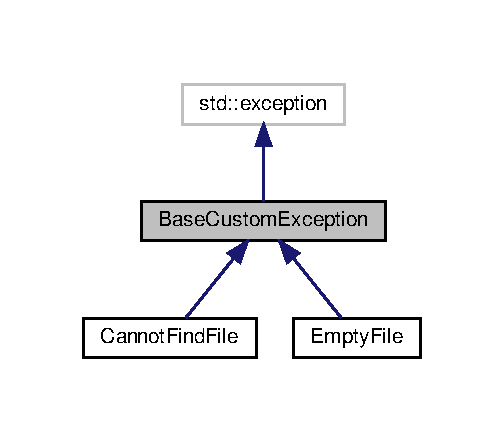
\includegraphics[width=242pt]{classBaseCustomException__inherit__graph}
\end{center}
\end{figure}


Collaboration diagram for Base\+Custom\+Exception\+:
\nopagebreak
\begin{figure}[H]
\begin{center}
\leavevmode
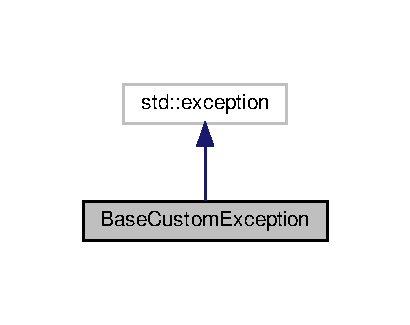
\includegraphics[width=197pt]{classBaseCustomException__coll__graph}
\end{center}
\end{figure}
\subsection*{Public Member Functions}
\begin{DoxyCompactItemize}
\item 
\mbox{\Hypertarget{classBaseCustomException_a55c28748e3f2aa06d3938ace39e17272}\label{classBaseCustomException_a55c28748e3f2aa06d3938ace39e17272}} 
virtual std\+::pair$<$ char $\ast$, char $\ast$ $>$ {\bfseries get\+Message} ()
\end{DoxyCompactItemize}


The documentation for this class was generated from the following file\+:\begin{DoxyCompactItemize}
\item 
/home/magdalena/neural\+\_\+network-\//neural\+Network/src/Exceptions.\+h\end{DoxyCompactItemize}

\hypertarget{classCannotFindFile}{}\section{Cannot\+Find\+File Class Reference}
\label{classCannotFindFile}\index{Cannot\+Find\+File@{Cannot\+Find\+File}}


Inheritance diagram for Cannot\+Find\+File\+:
\nopagebreak
\begin{figure}[H]
\begin{center}
\leavevmode
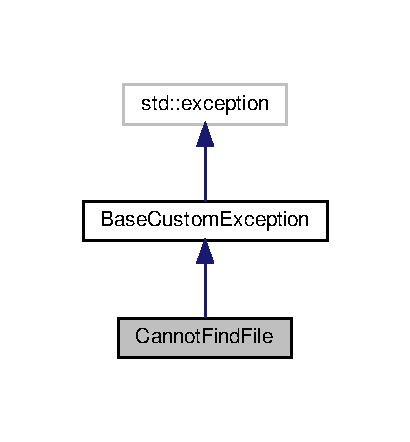
\includegraphics[width=197pt]{classCannotFindFile__inherit__graph}
\end{center}
\end{figure}


Collaboration diagram for Cannot\+Find\+File\+:
\nopagebreak
\begin{figure}[H]
\begin{center}
\leavevmode
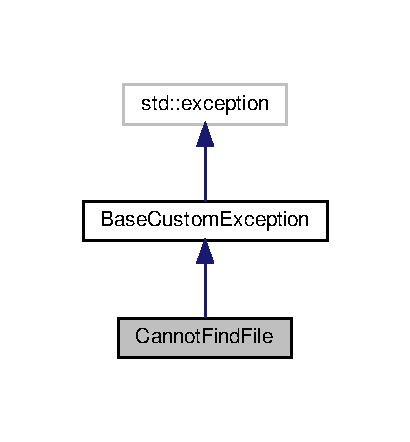
\includegraphics[width=197pt]{classCannotFindFile__coll__graph}
\end{center}
\end{figure}
\subsection*{Public Member Functions}
\begin{DoxyCompactItemize}
\item 
\mbox{\Hypertarget{classCannotFindFile_a1431a15fe56ddc4e7de6e2160c1f4447}\label{classCannotFindFile_a1431a15fe56ddc4e7de6e2160c1f4447}} 
std\+::pair$<$ char $\ast$, char $\ast$ $>$ {\bfseries get\+Message} ()
\end{DoxyCompactItemize}


The documentation for this class was generated from the following file\+:\begin{DoxyCompactItemize}
\item 
/home/magdalena/neural\+\_\+network-\//neural\+Network/src/Exceptions.\+h\end{DoxyCompactItemize}

\hypertarget{classEmptyFile}{}\section{Empty\+File Class Reference}
\label{classEmptyFile}\index{Empty\+File@{Empty\+File}}


Inheritance diagram for Empty\+File\+:
\nopagebreak
\begin{figure}[H]
\begin{center}
\leavevmode
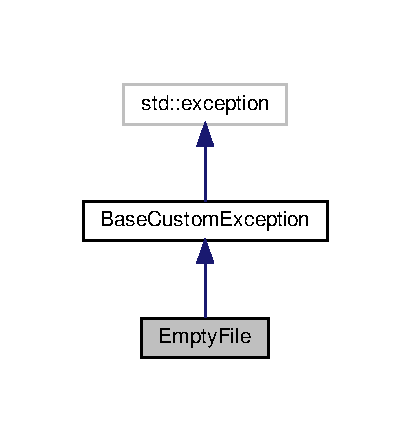
\includegraphics[width=197pt]{classEmptyFile__inherit__graph}
\end{center}
\end{figure}


Collaboration diagram for Empty\+File\+:
\nopagebreak
\begin{figure}[H]
\begin{center}
\leavevmode
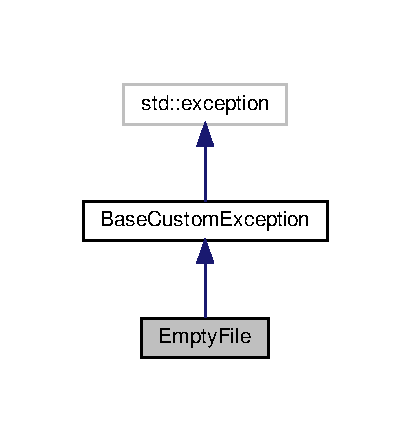
\includegraphics[width=197pt]{classEmptyFile__coll__graph}
\end{center}
\end{figure}
\subsection*{Public Member Functions}
\begin{DoxyCompactItemize}
\item 
\mbox{\Hypertarget{classEmptyFile_a94936a247d17ffd19005a191aa9f2a11}\label{classEmptyFile_a94936a247d17ffd19005a191aa9f2a11}} 
std\+::pair$<$ char $\ast$, char $\ast$ $>$ {\bfseries get\+Message} ()
\end{DoxyCompactItemize}


The documentation for this class was generated from the following file\+:\begin{DoxyCompactItemize}
\item 
/home/magdalena/neural\+\_\+network-\//neural\+Network/src/Exceptions.\+h\end{DoxyCompactItemize}

\hypertarget{classGUI}{}\section{G\+UI Class Reference}
\label{classGUI}\index{G\+UI@{G\+UI}}


Inheritance diagram for G\+UI\+:
\nopagebreak
\begin{figure}[H]
\begin{center}
\leavevmode
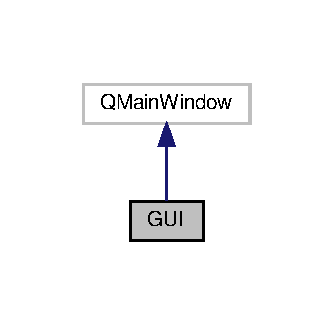
\includegraphics[width=160pt]{classGUI__inherit__graph}
\end{center}
\end{figure}


Collaboration diagram for G\+UI\+:
\nopagebreak
\begin{figure}[H]
\begin{center}
\leavevmode
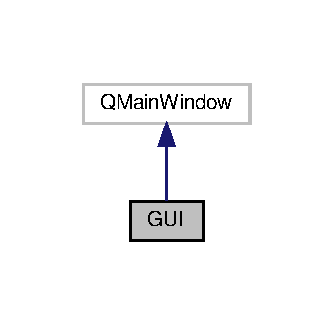
\includegraphics[width=160pt]{classGUI__coll__graph}
\end{center}
\end{figure}
\subsection*{Public Member Functions}
\begin{DoxyCompactItemize}
\item 
\mbox{\Hypertarget{classGUI_a15f66286a4f60a1af759ce6638a14c8a}\label{classGUI_a15f66286a4f60a1af759ce6638a14c8a}} 
{\bfseries G\+UI} (std\+::shared\+\_\+ptr$<$ \hyperlink{classNeuralNetworkImplementation}{Neural\+Network\+Implementation} $>$ pointer, Q\+Widget $\ast$parent=Q\+\_\+\+N\+U\+L\+L\+P\+TR)
\item 
\mbox{\Hypertarget{classGUI_a12302b586c0514055a96eb474ea7c50a}\label{classGUI_a12302b586c0514055a96eb474ea7c50a}} 
void {\bfseries print\+Logs} (std\+::string content)
\item 
\mbox{\Hypertarget{classGUI_a28c696839af97cd0ad977a8f1516ca89}\label{classGUI_a28c696839af97cd0ad977a8f1516ca89}} 
void {\bfseries print\+Error} (std\+::string content)
\item 
\mbox{\Hypertarget{classGUI_aa7df52281f532932c48fe873d34c3203}\label{classGUI_aa7df52281f532932c48fe873d34c3203}} 
void {\bfseries run\+Error\+Message\+Box} (std\+::pair$<$ char $\ast$, char $\ast$$>$ title\+And\+Message)
\end{DoxyCompactItemize}


The documentation for this class was generated from the following files\+:\begin{DoxyCompactItemize}
\item 
/home/magdalena/neural\+\_\+network-\//neural\+Network/src/\+G\+U\+I/G\+U\+I.\+h\item 
/home/magdalena/neural\+\_\+network-\//neural\+Network/src/\+G\+U\+I/G\+U\+I.\+cpp\end{DoxyCompactItemize}

\hypertarget{classUi_1_1GUIClass}{}\section{Ui\+:\+:G\+U\+I\+Class Class Reference}
\label{classUi_1_1GUIClass}\index{Ui\+::\+G\+U\+I\+Class@{Ui\+::\+G\+U\+I\+Class}}


Inheritance diagram for Ui\+:\+:G\+U\+I\+Class\+:
\nopagebreak
\begin{figure}[H]
\begin{center}
\leavevmode
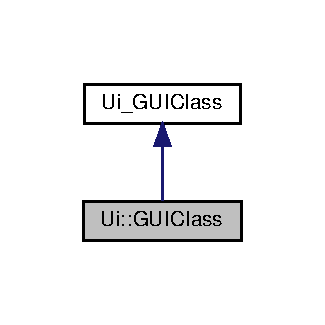
\includegraphics[width=156pt]{classUi_1_1GUIClass__inherit__graph}
\end{center}
\end{figure}


Collaboration diagram for Ui\+:\+:G\+U\+I\+Class\+:
\nopagebreak
\begin{figure}[H]
\begin{center}
\leavevmode
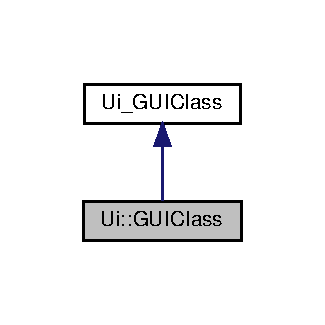
\includegraphics[width=156pt]{classUi_1_1GUIClass__coll__graph}
\end{center}
\end{figure}
\subsection*{Additional Inherited Members}


The documentation for this class was generated from the following file\+:\begin{DoxyCompactItemize}
\item 
/home/magdalena/neural\+\_\+network-\//neural\+Network/src/\+G\+U\+I/G\+U\+I1.\+h\end{DoxyCompactItemize}

\hypertarget{classLayer}{}\section{Layer Class Reference}
\label{classLayer}\index{Layer@{Layer}}
\subsection*{Public Member Functions}
\begin{DoxyCompactItemize}
\item 
\mbox{\Hypertarget{classLayer_a6cc1a7bfe1df555cfe2cf39fc5dae343}\label{classLayer_a6cc1a7bfe1df555cfe2cf39fc5dae343}} 
{\bfseries Layer} (int number\+Of\+Neurons, int number\+Of\+Inputs\+For\+One\+Percepton, bool offset\+For\+Firs\+Layer=false)
\item 
\mbox{\Hypertarget{classLayer_aac5b6143271ba7eac1bbfdf73ee5836a}\label{classLayer_aac5b6143271ba7eac1bbfdf73ee5836a}} 
std\+::vector$<$ double $>$ {\bfseries get\+Output\+From\+This\+Layer} (std\+::vector$<$ double $>$ \&output\+From\+Previous\+Layer)
\item 
\mbox{\Hypertarget{classLayer_ab2f29f66dd9d8364a2fc5ece4dd71536}\label{classLayer_ab2f29f66dd9d8364a2fc5ece4dd71536}} 
void {\bfseries step\+Backward} (double M\+SE, std\+::vector$<$ double $>$ \&input\+Values, double learning\+Rate)
\end{DoxyCompactItemize}


The documentation for this class was generated from the following files\+:\begin{DoxyCompactItemize}
\item 
/home/magdalena/neural\+\_\+network-\//neural\+Network/src/Layer.\+h\item 
/home/magdalena/neural\+\_\+network-\//neural\+Network/src/Layer.\+cpp\end{DoxyCompactItemize}

\hypertarget{classNeuralNetwork}{}\section{Neural\+Network Class Reference}
\label{classNeuralNetwork}\index{Neural\+Network@{Neural\+Network}}
\subsection*{Public Member Functions}
\begin{DoxyCompactItemize}
\item 
\mbox{\Hypertarget{classNeuralNetwork_a7181c2cefc064a45571bb456c4a8f862}\label{classNeuralNetwork_a7181c2cefc064a45571bb456c4a8f862}} 
{\bfseries Neural\+Network} (int number\+Of\+Layers, int number\+Of\+Input\+Neurons)
\item 
\mbox{\Hypertarget{classNeuralNetwork_a76b4eda80a260d3a712bab64033e022d}\label{classNeuralNetwork_a76b4eda80a260d3a712bab64033e022d}} 
double {\bfseries step\+Forward} (const std\+::vector$<$ double $>$ \&Input)
\item 
\mbox{\Hypertarget{classNeuralNetwork_addb381671a94934b406cc015328f9867}\label{classNeuralNetwork_addb381671a94934b406cc015328f9867}} 
void {\bfseries step\+Backward} (double M\+SE, const std\+::vector$<$ double $>$ \&input\+Values, double learning\+Rate)
\item 
\mbox{\Hypertarget{classNeuralNetwork_a7f87c803cd82de8c9ac626e6b9356fa3}\label{classNeuralNetwork_a7f87c803cd82de8c9ac626e6b9356fa3}} 
bool {\bfseries get\+Result} (std\+::vector$<$ double $>$ \&input\+Values)
\end{DoxyCompactItemize}


The documentation for this class was generated from the following files\+:\begin{DoxyCompactItemize}
\item 
/home/magdalena/neural\+\_\+network-\//neural\+Network/src/Neural\+Network.\+h\item 
/home/magdalena/neural\+\_\+network-\//neural\+Network/src/Neural\+Network.\+cpp\end{DoxyCompactItemize}

\hypertarget{classNeuralNetworkImplementation}{}\section{Neural\+Network\+Implementation Class Reference}
\label{classNeuralNetworkImplementation}\index{Neural\+Network\+Implementation@{Neural\+Network\+Implementation}}
\subsection*{Public Member Functions}
\begin{DoxyCompactItemize}
\item 
\mbox{\Hypertarget{classNeuralNetworkImplementation_ace88a14ae1b4b6549500a5bdb3338834}\label{classNeuralNetworkImplementation_ace88a14ae1b4b6549500a5bdb3338834}} 
{\bfseries Neural\+Network\+Implementation} (int number\+Of\+Layers, int number\+Of\+Input\+Neurons, std\+::string const \&data\+Filename, double desired\+Training\+Set\+Accuracy, double desired\+Training\+Set\+M\+SE, double alpha)
\item 
\mbox{\Hypertarget{classNeuralNetworkImplementation_a8ac321d48e1b24fece35f5efb3a7a598}\label{classNeuralNetworkImplementation_a8ac321d48e1b24fece35f5efb3a7a598}} 
std\+::string {\bfseries get\+Classification} (std\+::vector$<$ double $>$ \&input\+Data)
\item 
\mbox{\Hypertarget{classNeuralNetworkImplementation_a0eb89743ab3777a68ba60787db245ca0}\label{classNeuralNetworkImplementation_a0eb89743ab3777a68ba60787db245ca0}} 
std\+::string {\bfseries load\+Data\+And\+Train} ()
\end{DoxyCompactItemize}


The documentation for this class was generated from the following files\+:\begin{DoxyCompactItemize}
\item 
/home/magdalena/neural\+\_\+network-\//neural\+Network/src/Neural\+Network\+Implementation.\+h\item 
/home/magdalena/neural\+\_\+network-\//neural\+Network/src/Neural\+Network\+Implementation.\+cpp\end{DoxyCompactItemize}

\hypertarget{classPerceptron}{}\section{Perceptron Class Reference}
\label{classPerceptron}\index{Perceptron@{Perceptron}}
\subsection*{Public Member Functions}
\begin{DoxyCompactItemize}
\item 
\mbox{\Hypertarget{classPerceptron_a1d0126d97a8ffa9e67780a22614dd70e}\label{classPerceptron_a1d0126d97a8ffa9e67780a22614dd70e}} 
{\bfseries Perceptron} (int number\+Of\+Inputs, int offset\+For\+First\+Layer=0)
\item 
\mbox{\Hypertarget{classPerceptron_aa8481928b23d4c1193fe9a5be8be4f34}\label{classPerceptron_aa8481928b23d4c1193fe9a5be8be4f34}} 
double {\bfseries get\+Output} (std\+::vector$<$ double $>$ \&output\+From\+Previous\+Layer)
\item 
\mbox{\Hypertarget{classPerceptron_ab892c5f786ef0adc50a1c67714176ec6}\label{classPerceptron_ab892c5f786ef0adc50a1c67714176ec6}} 
double {\bfseries sigmoid} (double x)
\item 
\mbox{\Hypertarget{classPerceptron_ab875e1c9a1c95567679ac0cc8b8e2387}\label{classPerceptron_ab875e1c9a1c95567679ac0cc8b8e2387}} 
double {\bfseries linear} (double x)
\item 
\mbox{\Hypertarget{classPerceptron_a354a430917bbd8616231952690a4a542}\label{classPerceptron_a354a430917bbd8616231952690a4a542}} 
double {\bfseries get\+Weighted\+Input\+Value} (std\+::vector$<$ double $>$ \&output\+From\+Previous\+Layer)
\item 
\mbox{\Hypertarget{classPerceptron_a1be285519597daa4471b18f634f4c543}\label{classPerceptron_a1be285519597daa4471b18f634f4c543}} 
std\+::vector$<$ double $>$ {\bfseries get\+Weights} (\hyperlink{classPerceptron}{Perceptron} \&neuron)
\item 
\mbox{\Hypertarget{classPerceptron_ac3ec883408c075c35205a6d85f942ceb}\label{classPerceptron_ac3ec883408c075c35205a6d85f942ceb}} 
void {\bfseries step\+Backward} (double M\+SE, std\+::vector$<$ double $>$ \&input\+Values, double learning\+Rate)
\end{DoxyCompactItemize}


The documentation for this class was generated from the following files\+:\begin{DoxyCompactItemize}
\item 
/home/magdalena/neural\+\_\+network-\//neural\+Network/src/Perceptron.\+h\item 
/home/magdalena/neural\+\_\+network-\//neural\+Network/src/Perceptron.\+cpp\end{DoxyCompactItemize}

\hypertarget{classTrainingData}{}\section{Training\+Data Class Reference}
\label{classTrainingData}\index{Training\+Data@{Training\+Data}}
\subsection*{Public Member Functions}
\begin{DoxyCompactItemize}
\item 
\mbox{\Hypertarget{classTrainingData_a64e80f943b98acce134824f40689cfb8}\label{classTrainingData_a64e80f943b98acce134824f40689cfb8}} 
{\bfseries Training\+Data} (std\+::string const \&filename)
\item 
\mbox{\Hypertarget{classTrainingData_a4550118e30a983fb12158b54752445c8}\label{classTrainingData_a4550118e30a983fb12158b54752445c8}} 
int {\bfseries load\+Data} ()
\item 
\mbox{\Hypertarget{classTrainingData_a35b1501f0710acc3c402893a409ace6c}\label{classTrainingData_a35b1501f0710acc3c402893a409ace6c}} 
int {\bfseries get\+Size\+Of\+Data} ()
\item 
\mbox{\Hypertarget{classTrainingData_ad99f4428d6077419bb6a8452205693c0}\label{classTrainingData_ad99f4428d6077419bb6a8452205693c0}} 
int {\bfseries next\+Output\+Value} (double output)
\item 
\mbox{\Hypertarget{classTrainingData_a69f531f39a49988ef21b6fabfa06f82e}\label{classTrainingData_a69f531f39a49988ef21b6fabfa06f82e}} 
std\+::vector$<$ double $>$ {\bfseries get\+Data\+From\+One\+Row} (int idx)
\item 
\mbox{\Hypertarget{classTrainingData_ab5d2eb8782e49d7fe40d9261ae21d6e9}\label{classTrainingData_ab5d2eb8782e49d7fe40d9261ae21d6e9}} 
void {\bfseries split\+Data} ()
\item 
\mbox{\Hypertarget{classTrainingData_abeab409eacf5b0edfb5d1c1d9f18e552}\label{classTrainingData_abeab409eacf5b0edfb5d1c1d9f18e552}} 
std\+::vector$<$ double $>$ {\bfseries get\+Results} ()
\item 
\mbox{\Hypertarget{classTrainingData_a482f15e71cff8363debaf5a546be8b90}\label{classTrainingData_a482f15e71cff8363debaf5a546be8b90}} 
std\+::vector$<$ std\+::vector$<$ double $>$ $>$ {\bfseries get\+Inputs} ()
\end{DoxyCompactItemize}


The documentation for this class was generated from the following files\+:\begin{DoxyCompactItemize}
\item 
/home/magdalena/neural\+\_\+network-\//neural\+Network/src/Training\+Data.\+h\item 
/home/magdalena/neural\+\_\+network-\//neural\+Network/src/Training\+Data.\+cpp\end{DoxyCompactItemize}

\hypertarget{classUi__GUIClass}{}\section{Ui\+\_\+\+G\+U\+I\+Class Class Reference}
\label{classUi__GUIClass}\index{Ui\+\_\+\+G\+U\+I\+Class@{Ui\+\_\+\+G\+U\+I\+Class}}


Inheritance diagram for Ui\+\_\+\+G\+U\+I\+Class\+:
\nopagebreak
\begin{figure}[H]
\begin{center}
\leavevmode
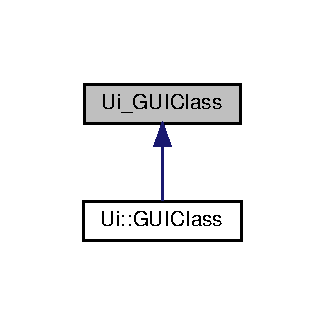
\includegraphics[width=156pt]{classUi__GUIClass__inherit__graph}
\end{center}
\end{figure}
\subsection*{Public Member Functions}
\begin{DoxyCompactItemize}
\item 
\mbox{\Hypertarget{classUi__GUIClass_a81ab1a446b71bd28a4bd7a7c78fe8e9f}\label{classUi__GUIClass_a81ab1a446b71bd28a4bd7a7c78fe8e9f}} 
void {\bfseries setup\+Ui} (Q\+Main\+Window $\ast$G\+U\+I\+Class)
\item 
\mbox{\Hypertarget{classUi__GUIClass_adb316b97c3459c7335479a71bbebd9de}\label{classUi__GUIClass_adb316b97c3459c7335479a71bbebd9de}} 
void {\bfseries retranslate\+Ui} (Q\+Main\+Window $\ast$G\+U\+I\+Class)
\end{DoxyCompactItemize}
\subsection*{Public Attributes}
\begin{DoxyCompactItemize}
\item 
\mbox{\Hypertarget{classUi__GUIClass_a35c6c14ea01041b996f3454aa9b0d715}\label{classUi__GUIClass_a35c6c14ea01041b996f3454aa9b0d715}} 
Q\+Action $\ast$ {\bfseries action\+New}
\item 
\mbox{\Hypertarget{classUi__GUIClass_a2f55de4b93fb2ad8cd15d62d722fab7f}\label{classUi__GUIClass_a2f55de4b93fb2ad8cd15d62d722fab7f}} 
Q\+Widget $\ast$ {\bfseries central\+Widget}
\item 
\mbox{\Hypertarget{classUi__GUIClass_ad8ebdb6389251700c7ff6e739d998b43}\label{classUi__GUIClass_ad8ebdb6389251700c7ff6e739d998b43}} 
Q\+Grid\+Layout $\ast$ {\bfseries grid\+Layout\+\_\+4}
\item 
\mbox{\Hypertarget{classUi__GUIClass_a0691bb4c43e7aba13b83d5d427c8e7db}\label{classUi__GUIClass_a0691bb4c43e7aba13b83d5d427c8e7db}} 
Q\+Group\+Box $\ast$ {\bfseries Parameters\+Group\+Box}
\item 
\mbox{\Hypertarget{classUi__GUIClass_a5fae695f1e164527009a0d36998bbf5f}\label{classUi__GUIClass_a5fae695f1e164527009a0d36998bbf5f}} 
Q\+Grid\+Layout $\ast$ {\bfseries grid\+Layout\+\_\+2}
\item 
\mbox{\Hypertarget{classUi__GUIClass_a76794c0d518c5962f2ef259631905b3f}\label{classUi__GUIClass_a76794c0d518c5962f2ef259631905b3f}} 
Q\+Line\+Edit $\ast$ {\bfseries Marginal\+Adhesion\+Line\+Edit}
\item 
\mbox{\Hypertarget{classUi__GUIClass_a328408cec3a258c22f1e27a8176b508f}\label{classUi__GUIClass_a328408cec3a258c22f1e27a8176b508f}} 
Q\+Label $\ast$ {\bfseries Cell\+Size\+Label}
\item 
\mbox{\Hypertarget{classUi__GUIClass_aa5460635bb1d3dfb7a96fdadf9ff4818}\label{classUi__GUIClass_aa5460635bb1d3dfb7a96fdadf9ff4818}} 
Q\+Line\+Edit $\ast$ {\bfseries Cell\+Size\+Line\+Edit}
\item 
\mbox{\Hypertarget{classUi__GUIClass_a2a7a4ec6a8edef50d78949f7d79d9b49}\label{classUi__GUIClass_a2a7a4ec6a8edef50d78949f7d79d9b49}} 
Q\+Label $\ast$ {\bfseries Clump\+Thickness\+Label}
\item 
\mbox{\Hypertarget{classUi__GUIClass_a886316f7274680822ab608648eaba5f8}\label{classUi__GUIClass_a886316f7274680822ab608648eaba5f8}} 
Q\+Label $\ast$ {\bfseries Marginal\+Adhesion\+Label}
\item 
\mbox{\Hypertarget{classUi__GUIClass_aaab8a296384f757efff0e9eeddff7c5b}\label{classUi__GUIClass_aaab8a296384f757efff0e9eeddff7c5b}} 
Q\+Label $\ast$ {\bfseries Cell\+Shape\+Label}
\item 
\mbox{\Hypertarget{classUi__GUIClass_a8c91eee31e083df696a01b2937311cfc}\label{classUi__GUIClass_a8c91eee31e083df696a01b2937311cfc}} 
Q\+Line\+Edit $\ast$ {\bfseries Cell\+Shape\+Line\+Edit}
\item 
\mbox{\Hypertarget{classUi__GUIClass_aa4b338c827cd8c0db0c943638ebc87af}\label{classUi__GUIClass_aa4b338c827cd8c0db0c943638ebc87af}} 
Q\+Line\+Edit $\ast$ {\bfseries Bland\+Chromatin\+Line\+Edit}
\item 
\mbox{\Hypertarget{classUi__GUIClass_a02a0c8407a4fcf0c657d03a2ef09bd10}\label{classUi__GUIClass_a02a0c8407a4fcf0c657d03a2ef09bd10}} 
Q\+Label $\ast$ {\bfseries Mitoses\+Label}
\item 
\mbox{\Hypertarget{classUi__GUIClass_ab9c4178ebd3e4e015e99eef71161fbf6}\label{classUi__GUIClass_ab9c4178ebd3e4e015e99eef71161fbf6}} 
Q\+Line\+Edit $\ast$ {\bfseries Bare\+Nuclei\+Line\+Edit}
\item 
\mbox{\Hypertarget{classUi__GUIClass_ac435c33f89dfa69b7e5e6f5c984a16a9}\label{classUi__GUIClass_ac435c33f89dfa69b7e5e6f5c984a16a9}} 
Q\+Label $\ast$ {\bfseries Normal\+Nucleoli\+Label}
\item 
\mbox{\Hypertarget{classUi__GUIClass_a7cbd8d828cc6443f80c30c9fc818b510}\label{classUi__GUIClass_a7cbd8d828cc6443f80c30c9fc818b510}} 
Q\+Line\+Edit $\ast$ {\bfseries Mitoses\+Line\+Edit}
\item 
\mbox{\Hypertarget{classUi__GUIClass_a815914e062d8a0bbee6674fe74b52706}\label{classUi__GUIClass_a815914e062d8a0bbee6674fe74b52706}} 
Q\+Line\+Edit $\ast$ {\bfseries Epithelial\+Cell\+Size\+Line\+Edit}
\item 
\mbox{\Hypertarget{classUi__GUIClass_a4431cb7d00e0fa3bbb98dbafacf4f83e}\label{classUi__GUIClass_a4431cb7d00e0fa3bbb98dbafacf4f83e}} 
Q\+Label $\ast$ {\bfseries Bland\+Chromatin\+Label}
\item 
\mbox{\Hypertarget{classUi__GUIClass_ade9289c547f0d383982a907f5ea429ac}\label{classUi__GUIClass_ade9289c547f0d383982a907f5ea429ac}} 
Q\+Line\+Edit $\ast$ {\bfseries Clump\+Thickness\+Line\+Edit}
\item 
\mbox{\Hypertarget{classUi__GUIClass_af448163760b77e63dc6687e4961bb1c9}\label{classUi__GUIClass_af448163760b77e63dc6687e4961bb1c9}} 
Q\+Label $\ast$ {\bfseries Bare\+Nuclei\+Label}
\item 
\mbox{\Hypertarget{classUi__GUIClass_ac1aa1919b0b6d200cb5ee023f7afd84e}\label{classUi__GUIClass_ac1aa1919b0b6d200cb5ee023f7afd84e}} 
Q\+Line\+Edit $\ast$ {\bfseries Normal\+Nucleoli\+Line\+Edit}
\item 
\mbox{\Hypertarget{classUi__GUIClass_a57c6e1114411b0648fa6f64294f51b40}\label{classUi__GUIClass_a57c6e1114411b0648fa6f64294f51b40}} 
Q\+Label $\ast$ {\bfseries Epithelial\+Cell\+Size\+Label}
\item 
\mbox{\Hypertarget{classUi__GUIClass_a79ef34f1e52a3a2b793f5c26ab512228}\label{classUi__GUIClass_a79ef34f1e52a3a2b793f5c26ab512228}} 
Q\+Frame $\ast$ {\bfseries Push\+Buttons\+Frame}
\item 
\mbox{\Hypertarget{classUi__GUIClass_a35d8d50ebb378cc4ec46f6554f5f5dcf}\label{classUi__GUIClass_a35d8d50ebb378cc4ec46f6554f5f5dcf}} 
Q\+Grid\+Layout $\ast$ {\bfseries grid\+Layout\+\_\+3}
\item 
\mbox{\Hypertarget{classUi__GUIClass_a2f598ce2e9d7d620fd35138348becced}\label{classUi__GUIClass_a2f598ce2e9d7d620fd35138348becced}} 
Q\+Push\+Button $\ast$ {\bfseries Run\+Process\+Push\+Button}
\item 
\mbox{\Hypertarget{classUi__GUIClass_a28c34718ca00c228e5827e49ddbd385e}\label{classUi__GUIClass_a28c34718ca00c228e5827e49ddbd385e}} 
Q\+Frame $\ast$ {\bfseries Logs\+Frame}
\item 
\mbox{\Hypertarget{classUi__GUIClass_a9f3baf74e29941ecaaf1a65aa17ed55f}\label{classUi__GUIClass_a9f3baf74e29941ecaaf1a65aa17ed55f}} 
Q\+Grid\+Layout $\ast$ {\bfseries grid\+Layout}
\item 
\mbox{\Hypertarget{classUi__GUIClass_aa4aab8f8a82e885c79f370fd10f0a228}\label{classUi__GUIClass_aa4aab8f8a82e885c79f370fd10f0a228}} 
Q\+Label $\ast$ {\bfseries Logs\+Label}
\item 
\mbox{\Hypertarget{classUi__GUIClass_a227235f6ed633f00900eccf82beaed52}\label{classUi__GUIClass_a227235f6ed633f00900eccf82beaed52}} 
Q\+Push\+Button $\ast$ {\bfseries Clear\+Logs\+Push\+Button}
\item 
\mbox{\Hypertarget{classUi__GUIClass_a1e5223eadc39d1b2ad2c095ef8ec2b1a}\label{classUi__GUIClass_a1e5223eadc39d1b2ad2c095ef8ec2b1a}} 
Q\+Text\+Edit $\ast$ {\bfseries Logs\+Text\+Edit}
\item 
\mbox{\Hypertarget{classUi__GUIClass_aba670b52e0772bea7de163eb4316648e}\label{classUi__GUIClass_aba670b52e0772bea7de163eb4316648e}} 
Q\+Menu\+Bar $\ast$ {\bfseries menu\+Bar}
\item 
\mbox{\Hypertarget{classUi__GUIClass_ab990cb0e59c3184f5542e5c5564c8cf2}\label{classUi__GUIClass_ab990cb0e59c3184f5542e5c5564c8cf2}} 
Q\+Menu $\ast$ {\bfseries menu\+File}
\item 
\mbox{\Hypertarget{classUi__GUIClass_ae48af47c2edd5057a1836e5b872d8784}\label{classUi__GUIClass_ae48af47c2edd5057a1836e5b872d8784}} 
Q\+Tool\+Bar $\ast$ {\bfseries main\+Tool\+Bar}
\item 
\mbox{\Hypertarget{classUi__GUIClass_a54aefdd0673d1031847778a560fc14c4}\label{classUi__GUIClass_a54aefdd0673d1031847778a560fc14c4}} 
Q\+Status\+Bar $\ast$ {\bfseries status\+Bar}
\end{DoxyCompactItemize}


The documentation for this class was generated from the following file\+:\begin{DoxyCompactItemize}
\item 
/home/magdalena/neural\+\_\+network-\//neural\+Network/src/\+G\+U\+I/G\+U\+I1.\+h\end{DoxyCompactItemize}

%--- End generated contents ---

% Index
\backmatter
\newpage
\phantomsection
\clearemptydoublepage
\addcontentsline{toc}{chapter}{Index}
\printindex

\end{document}
